\documentclass[12pt]{amsart}
\usepackage{geometry}
\usepackage{amsmath}
\usepackage{amssymb}
\usepackage{graphicx}
\usepackage{subfig}
\usepackage[table]{xcolor}
\usepackage{color}
\usepackage{natbib}


\geometry{letterpaper}

%\usepackage[T1]{fontenc}

% general commands
\definecolor{lemonchiffon}{rgb}{1, .98, .80}
\definecolor{lightgrass}{rgb}{.89, 1, .87}
\newcommand{\vect}[1]{\boldsymbol{\mathbf{#1}}}
\newcommand{\degree}[1]{${#1}^{\circ}$}
\newcommand{\highlight}{ \rowcolor{lightgrass} }
\newcommand{\script}[1]{\mathcal{#1}}

\newcommand{\eqn}[1]{\begin{align*}
#1
\end{align*}}
\newcommand{\eqnl}[2]{\begin{align} \label{#1}
#2
\end{align}}
\newcommand{\shblock}{\hspace{3mm}}
\newcommand{\hblock}{\hspace{8mm}}
\newcommand{\eqnsep}{\shblock\hblock}

\newcommand{\bl}{\big\{}
\newcommand{\br}{\big\}}
\newcommand{\Bl}{\Big\{}
\newcommand{\Br}{\Big\}}


\newcommand{\indicator}{\mathbf{1}}

\newcommand{\mtx}[4]{
\[
#1 = #2
\left[ {\begin{array}{#3}
 #4
 \end{array} } \right]
\]
}

\newcommand{\eqnset}[4]{
\[ #1 = #2 \left\{ \begin{array}{#3}
        #4
\end{array} \right. \] 
}



        
        
        
        

% paper specific terms
\newcommand{\vz}{\vect{z}}
\newcommand{\vx}{\vect{x}}
\newcommand{\vy}{\vect{y}}
\newcommand{\vp}{\vect{\pi}}
\newcommand{\vph}{\hat{\vect{\pi}}}



\newcommand{\fab}{f_j}
\newcommand{\llp}{l(\vect{\pi})}
\newcommand{\llpp}{l(\vect{\pi^\prime})}


\newcommand{\hessll}[2]{\sumn \frac{f_{#1}}{(\summ \pi_j f_j)^2 f_{#2}}}
\newcommand{\hessllg}[2]{\sumn \frac{f_{#1}}{(\sumg \pi_j f_j)^2 f_{#2}}}
\newcommand{\hesslld}[2]{\frac{\partial^2 \llpp}{\partial \pi_{#1} \partial \pi_{#2}}}


\newcommand{\sumn}{\sum^n_{i=1}}
\newcommand{\summ}{\sum^m_{j=1}}
\newcommand{\sumg}{\sum^g_{j=1}}
\newcommand{\sumk}{\sum^m_{k=1}}


\newcommand{\img}[2]{
	\begin{figure}
		\centering
		\includegraphics[width=\textwidth]{#1}
		\caption{#2}
	\end{figure}
}

\newcommand{\imgi}[1]{
	\vspace{10mm}
	\includegraphics[width=\textwidth]{#1}
	\vspace{10mm}
}

%%% TITLE
\title{Metallicity}
\author{\today}

%%% BEGIN DOCUMENT
\begin{document}

\maketitle






%%%%%%%%%%%%%%%%%%%%%%%%%%%%%%%%%%%%%%%%%%%%%%%%%%%%%%
\section{Mixture model}

For each observation of ($L, \frac{\alpha}{\text{Fe}}, \frac{\text{Fe}}{\text{H}})$, let $\bl (x_i,y_i) \br^n_{i=1}$ represent observed metallicities of stars drawn from one of $m$ known model densities. We model the density of observations using the mixture model

\eqn{
	f(x,y) = \summ \pi_j \fab(x,y) \eqnsep \summ \pi_j = 1 \eqnsep \pi_j \geq 0, j=1,\ldots,m
}

With a complete likelihood of

\eqn{
	L(\vect{\pi}) &= \prod^n_{i=1} f(x_i,y_i)	 = \prod^n_{i=1} \Bl  \summ \pi_j \fab(x_i,y_i)  \Br	\\
	\llp &= \sumn \log \Big( \summ \pi_j \fab(x_i,y_i)  \Big)
}

Evaluation of $\partial l(\vect{\pi})/\partial \pi$ can be avoided by adding a latent indicator, $z$, to the observed data $(x,y)$, representing the model group from which that observation was generated. Let $G_j$ be the $j^\text{th}$ model group, and let

\eqn{z_{ij} = \indicator \bl (x_i,y_i) \mapsto G_j \br}


The incomplete data likelihood is defined over the complete data $\bl (x_i,y_i,\vect{z}_i) \br^n_{i=1}$ as

\eqn{
	L(\vect{\pi}) &= \prod^n_{i=1} \prod^m_{j=1} \Bl \fab(x_i,y_i) \Br ^{z_{ij}} \pi_j^{z_{ij}}	\\
	\llp &= \sumn \summ z_{ij}  \log \bl \pi_j  \fab(x_i,y_i) \br
}





%%%%%%%%%%%%%%%%%%%%%%%%%%%%%%%%%%%%%%%%%%%%%%%%%%%%%%
\clearpage
\section{EM}

First we find the expected value of $\llp$ conditional on the distribution of z. Since $z_{ij}$ is an indicator function, its expected value is equal to the probability that data point $i$ comes from model $j$.

\subsection{Expected value of $\llp$}
The expected value of  $\llp$ is

\eqn{
	\text{E}_{\vp}\Big[\llp \big| \vx,\vy \Big] &= \sumn E(\vp | x_i, y_i) l(\vp | x_i, y_i) 		\\
	&= \sumn \summ E_{\vp}\big[z_{ij}|x_i,y_i\big] \bl \log \fab(x_i,y_i) + \log \pi_j  \br
}

where
\eqn{
	\text{E}_{\vp}\Big[  z_{ij} | x_i, y_i \Big] = \text{Probability}\Big((x_i,y_i) \mapsto G_j \big | x_i,y_i\Big)
}








\subsection{Expected value of $\pi|\vect{x},\vect{y}$}
The expected value of $z_{ij}$ is the same as the expected value of $\pi_j$, given the data. This can be specified as

\eqn{
	\text{E}_{\vp}\Big[ z_{j} | x_i,y_i \Big] = P(z_j|x_i,y_i) = \frac{P(x_i,y_i|z_j=1)P(z_j=1)}{P(x_i,y_i)}
}

with constituent parts:
\eqn{
	P(x_i,y_i | z_j=1) = f_j(x_i,y_i) \eqnsep  P(x_i,y_i|z_j) = \prod^m_{j=1}f_j^{z_i}	 \eqnsep  P(z_j) = \prod^m_{j=1} \pi_j^{z_j}
}

thus
\eqn{
	\text{E}_{\vp}\Big[ z_{j} | x_i,y_i \Big] &=  \frac{\pi_j \fab(x_i,y_i)}{\summ \pi_j \fab(x_i,y_i)}
}


Defining $w^{(t)}_{ij}$ as the expected value of $z_{ij}$ at the $t^\text{th}$ step, and $\pi^{(t)}_j$ as the MLE of $\pi_j$  at the $t^\text{th}$ step, yeilds
\eqn{
	w^{(t+1)}_{ij} &= \frac{\pi^{(t)}_{j} \fab(x_i,y_i)}{\sumk \pi^{(t)}_{k}f_k(x_i,y_i)}
}







\subsection{Solving for $\vp$}
\eqn{
	0 &= \frac{\partial}{\partial \pi_k} \text{E}_{\vect{\pi}}\Big[\llp \big| \vect{x},\vect{y}\Big]    \\
	& =      \sumn \Bl  w^{(0)}_{ij} \frac{1}{\pi_k} - w^{(0)}_{im} \frac{1}{1-\pi_1-\ldots-\pi_{m-1}}   \Br, k=1,\ldots,m-1
}

Therefore


\eqn{
	\frac{1}{\pi_1} \sumn w^{(0)}_{i1} &= \ldots = \frac{1}{\pi_{m-1}} \sumn w^{(0)}_{i,m-1} = c	\\
	\hat{\pi}_k &= \frac{\sumn w^{(0)}_{ik}}{c}		\\
	\pi^{(1)}_j &= \frac{\sumn w^{(0)}_{ij}}{n}
}

And in general,


\eqn{
	\pi^{(t+1)}_j = \frac{\sumn w^{(t)}_{ij}}{n}
}




%%%%%%%%%%%%%%%%%%%%%%%%%%%%%%%%%%%%%%%%%%%%%%%%%%%%%%
\clearpage
\section{Observed Information}

As $\pi_m = 1-\summ \pi_j$ there are only $g$ free parameters. Thus let $g=m-1$, and $\vp^\prime=\vp[1,\ldots,g]$. The observed information matrix, $I(\vp^\prime|\vx,\vy)$ is given by the $g\times g$ negative hessian:

\eqn{
	\llpp &= \sumn \log \Big( \sumg \pi_j \fab  \Big)		\\
	\frac{\partial \llpp}{\partial \pi_k} &= \sumn \frac{f_k}{\sumg \pi_j f_j}	\\
	\frac{\partial^2 \llpp}{\partial \pi_k \partial \pi_r} &= -\sumn \frac{f_k}{(\sumg \pi_j f_j)^2 f_r}
}

\mtx{I(\vp|\vx,\vy)=-\frac{\partial^2 \llpp}{\partial \vp^\prime \partial \vp^{\prime T}}}{-}{cccc}{
	\frac{\partial^2 \llpp}{\partial \pi_1^2} & \hesslld{1}{2} & \ldots & \hesslld{1}{g}	\\
	\vdots & \vdots & & \vdots	\\
	\hesslld{g}{1} & \hesslld{g}{2} & \ldots & \frac{\partial^2 \llpp}{\partial \pi_{g}^2}
}

\mtx{}{}{cccc}{
	\sumn \frac{1}{(\sumg \pi_j f_j)^2} & \hessllg{1}{2} & \ldots & \hessllg{1}{g}	\\
	\vdots & \vdots & & \vdots	\\
	\hessllg{g}{1} & \hessllg{g}{2} & \ldots & \sumn \frac{1}{(\sumg \pi_j f_j)^2}
}

*Excluding $i$ where $(\sumg \pi_j f_j)^2 f_{i}=0$ to avoid dividing by zero.

\subsection{Variance and Covariance of $\vp$}
The asymptotic covariance matrix of $\vp$ can be approximated by the inverse of the observed information matrix, $I^{-1}(\vph|\vx,\vy)$, yielding

\eqnset{\text{Cov}(\pi_p,\pi_q)}{}{ll}{
	I^{-1}(\vph) 				& p,q<m	\\
	\sum\limits_{j=1}^g \text{Cov}(\pi_j,\pi_q)		& p=m,q<m	\\
	\sum\limits_{j=1}^g \sum\limits_{k=1}^g \text{Cov}(\pi_j,\pi_k)		& p, q=m	\\
}

\eqn{
	\text{Var}(\pi_j) &= \sigma^2_j = \Bl \big | \text{Cov}(\vp) \big | \Br_{jj}
}
* There are many negative covariances; this is ok I think.



\begin{center}
	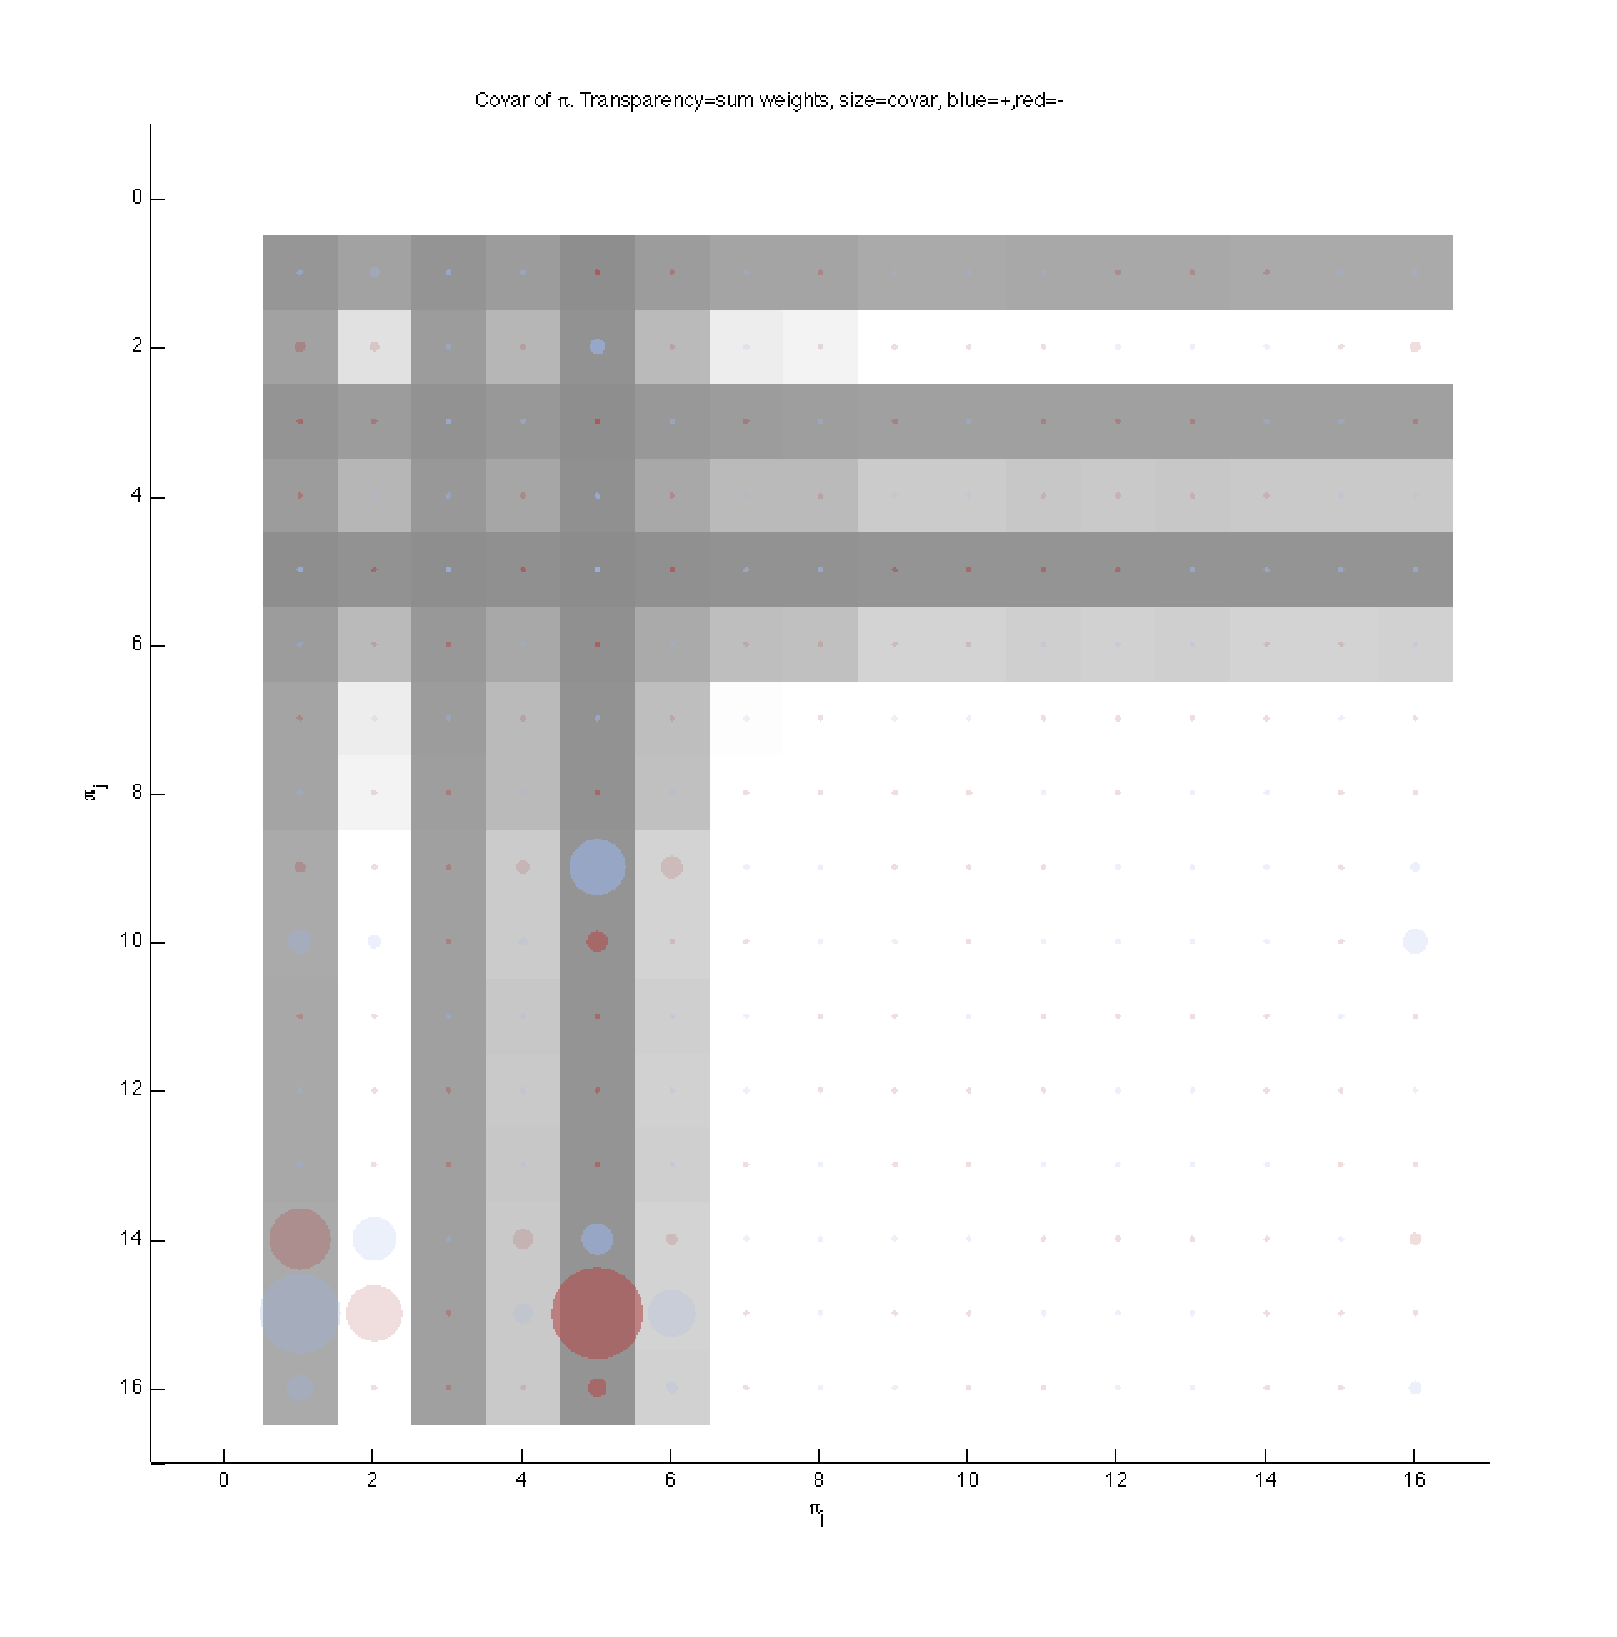
\includegraphics[scale=0.42]{covar.pdf}
\end{center}


\begin{table}[h]\tiny
\caption{Covariance, in percent, of $\vph$ overlaid on $\hat{\pi}_i + \hat{\pi}_j$. Larger dots are covariances; negative covariances are red.}
	\begin{center}
		\begin{tabular}{r r r r r r r r r r r r r r r r}
			 0.0001   &     0.001    &       -  &        -  &   -0.0004   &   -0.0001   &        -  &        -   &   0.0001     &      -     &     -  &        -  &        -  &        -    &      -   &   0.0007         \\
 -0.001   &   -0.0009    &       -  &   -0.0002   &    0.0015   &   -0.0004   &        -  &        -   &       -    &      -     &     -  &        -  &        -  &        -    &      -   &   -0.001         \\
     -  &        -   &       -  &        -  &        -  &        -  &        -  &        -   &       -    &      -     &     -  &        -  &        -  &        -    &      -   &       -        \\
-0.0002   &    0.0003    &       -  &        -  &        -  &        -  &        -  &        -   &       -    &      -     &     -  &        -  &        -  &        -    &      -   &       -        \\
     -  &   -0.0001    &       -  &        -  &    0.0001   &        -  &        -  &        -   &       -    &      -     &     -  &        -  &        -  &        -    &      -   &       -        \\
 0.0003   &   -0.0001    &       -  &    0.0001   &   -0.0004   &    0.0002   &        -  &        -   &       -    &      -     &     -  &        -  &        -  &        -    &      -   &       -        \\
-0.0001   &        -   &       -  &        -  &        -  &        -  &        -  &        -   &       -    &      -     &     -  &        -  &        -  &        -    &      -   &       -        \\
     -  &        -   &       -  &        -  &        -  &        -  &        -  &        -   &       -    &      -     &     -  &        -  &        -  &        -    &      -   &       -        \\
-0.0011   &   -0.0001    &       -  &   -0.0013   &    0.0053   &   -0.0021   &        -  &        -   &       -    &      -     &     -  &        -  &        -  &    0.0001     &      -   &    0.001         \\
 0.0023   &    0.0013    &  -0.0001   &    0.0008   &    -0.002   &        -  &   -0.0001   &    0.0001    &       -    &      -     &     -  &        -  &        -  &        -    &      -   &   0.0023         \\
     -  &        -   &       -  &        -  &   -0.0001   &    0.0001   &        -  &        -   &       -    &      -     &     -  &        -  &        -  &        -    &      -   &       -        \\
     -  &        -   &       -  &        -  &        -  &        -  &        -  &        -   &       -    &      -     &     -  &        -  &        -  &        -    &      -   &       -        \\
 0.0003   &   -0.0003    &       -  &        -  &   -0.0001   &    0.0001   &        -  &        -   &       -    &      -     &     -  &        -  &        -  &        -    &      -   &       -        \\
-0.0058   &    0.0041    &   0.0001   &   -0.0019   &     0.003   &   -0.0011   &    0.0002   &    0.0001    &   0.0003     &      -     &     -  &   -0.0001   &   -0.0001   &   -0.0001     &      -   &  -0.0012         \\
 0.0076   &   -0.0053    &  -0.0001   &    0.0019   &   -0.0086   &    0.0045   &   -0.0003   &    0.0002    &  -0.0003     &      -     &     -  &        -  &        -  &   -0.0001     &      -   &  -0.0005         \\
 0.0025   &   -0.0001    &  -0.0001   &   -0.0005   &   -0.0018   &    0.0011   &   -0.0001   &    0.0003    &       -    &      -     &     -  &        -  &        -  &        -    &      -   &   0.0012         \\	
		\end{tabular}
	\end{center}
\end{table}


 
\begin{figure}
  \centering
  \subfloat[Larger dots represent more weight accounted for by that $\hat{\pi}_j$.]{ \raisebox{-40mm}{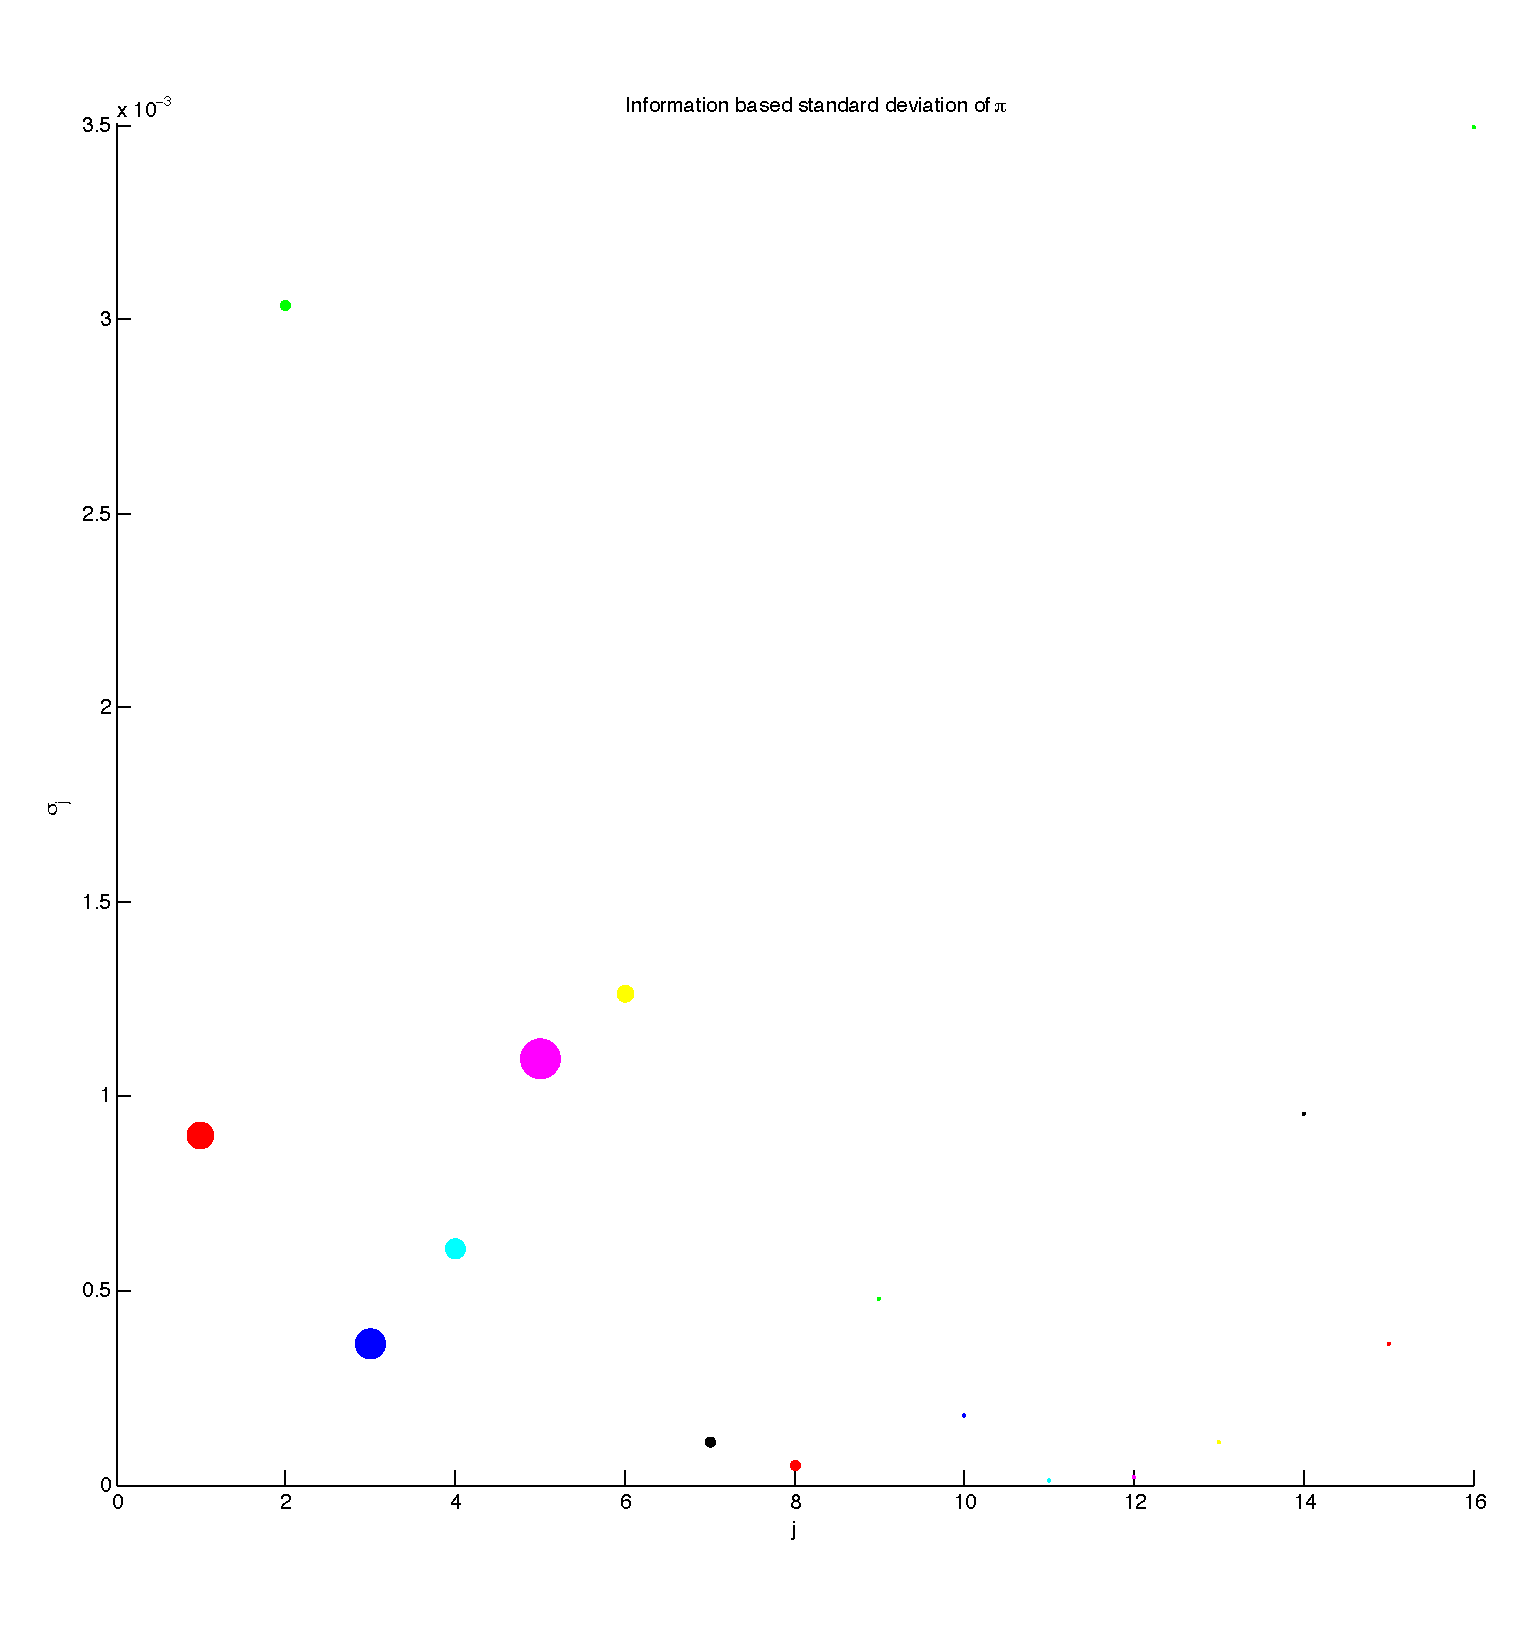
\includegraphics[scale=0.3]{stdev.pdf}}}                
  \subfloat[]{\begin{tabular}{r| r| r| r| r|}
		& $\hat{\pi}_j$ & $\pi_j$ & $\sigma_{\hat{\pi}_j}$ & Z-score	\\
		\hline
1	&	16.04  &		14.467   &	0.0898  &	17.509			\\
2	&	 3.320 &		 7.435   &	0.3033  &  -13.564			\\
3	&	21.392 &		20.991   &	0.0361  &	11.067			\\
4	&	 8.846 &		 9.234   &	0.0608  &	-6.369			\\
5	&	36.443 &		33.656   &	0.1094  &	25.479			\\
6	&	 7.882 &		 8.019   &	0.1264  &	-1.080			\\
7	&	 2.560 &		 2.400   &	0.0108  &	14.793			\\
8	&	 2.239 &		 2.573   &	0.0047  &  -70.08 			\\
9	&	 0	&    	 0.118   	&	0.0480  &	-2.474			\\
10	&	 0	&    	 0.076   	&	0.0178  &	-4.317			\\
11	&	 0.421   &	 0.358   	&	0.0009	&	65.245			\\
12	&	 0.246   &	 0.253   	&	0.0021  &	-2.959			\\
13	&	 0.485   &	 0.225   	&	0.0110  &	23.56 			\\
14	&	 0.008 	& 	 0.048   	&	0.0954  &	-0.420	\\
15	&	 0.030   &	 0.024	&		0.0362  &	 0.183	\\
16	&	 0.083   &	 0.046	&		0.3494  &	 0.103	\\
   		\end{tabular}}
  \caption{Variance of $\vph$, true $\vp$, in percent, and z-scores.}
\end{figure}






\eqn{
	\text{Z-score} = \frac{\hat{\pi}_j - \pi}{\sigma_{\hat{\pi}_j}}
}
               
               
               
               

%%%%%%%%%%%%%%%%%%%%%%%%%%%%%%%%%%%%%%%%%%%%%%%%%%%%%%
\clearpage
\section{Likelihood ratio test}
Given certain conditions
\eqn{
	H_0: \vp = \vp_\text{true}	\\
	H_1: \vp \neq \vp_\text{true}
}

\eqn{
	\Lambda = -2 \log \frac{ \sup_{\vp=\vp_\text{true}} \llp}{ \sup_{\vp} \llp }  = -2\bl l(\vp_\text{true}) - l(\vph) \br \sim \chi^2_{m-1}	\\
}
\eqn{
	\Lambda_\text{Halo 3} &= 25.025 \sim \chi^2_{15}	\\
	\text{p-value 10k} &= 4.961\%\\
	\text{p-value 30k} &= 1.3\times 10^{-5}\%\\
	\text{p-value 50k} &= 1.4\times 10^{-12}\%
}

Thus we accept $H_0$ when requiring 95\% or less confidence; there is only a 4.961\% chance we would see a value this extreme or more given $H_0$ is true. This holds for 400 to 1600 EM iterations.







\end{document}











%%%%%%%%%%%%%%%%%%%%%%%%%%%%%%%%%%%%%%%%%%%%%%%%%%%%%%
\clearpage
\section{Other}
\subsection{Convergence}
$\llp$ from 1.235 to 1.236 over past 25 runs is the slowest rate of convergence.

\subsection{To do}
Bias, consistency, efficiency, method of moments, $\sigma$ as a function of n. Bootstrapping, n+1 bootstrapping as a check that n is large enough for fisher info.


MAP 2.8.5.

Alt T 2.7.3.

basis of test 2.7.1.

deterministic annealing em algo 2.12.4.

stochiastic em 2.13.

conditional bootstrap 2.15.5. 


alt approach to fisher info: 2.16.1: using wald and reduced parameter holding out.

full bootstrap 2.16.2



2.18.2 modified lrt

2.18.1 outliers

2.19 partial classification

3.5

3.8.1


spectral decomposition: 3.12.1

k means classification for auto binning?

4: mcmc for mixture

5.5.2: exactly what we did--nonormal

5.5.4: mulitcycle

5.13 hierarchical mixtures of experts


6.13 skewness of lrt and m

6.3.2

6.5

6.6 bootstrapping lrts

6.7 pval boots

6.7.2 double boots

6.8 bias corr for log like, aic, boots info, cv info

6.9 bayeseian info

6.10 classification based info

9 fitting mix to bin data

11 mix analys of directional data

13 hidden markov models
















